%% This is file `prletters-template.tex',
%% 
%% Copyright 2013 Elsevier Ltd
%% 
%% This file is part of the 'Elsarticle Bundle'.
%% ---------------------------------------------
%% 
%% It may be distributed under the conditions of the LaTeX Project Public
%% License, either version 1.2 of this license or (at your option) any
%% later version.  The latest version of this license is in
%%    http://www.latex-project.org/lppl.txt
%% and version 1.2 or later is part of all distributions of LaTeX
%% version 1999/12/01 or later.
%% 
%% The list of all files belonging to the 'Elsarticle Bundle' is
%% given in the file `manifest.txt'.
%% 
%% Template article for Elsevier's document class `elsarticle'
%% with harvard style bibliographic references
%%
%% $Id: prletters-template-with-authorship.tex 69 2013-07-15 10:15:25Z rishi $
%%
%% This template has no review option
%% 
%% Use the options `twocolumn,final' to obtain the final layout
\documentclass[times,twocolumn,final,authoryear]{elsarticle}

%% Stylefile to load PR Letters template
\usepackage{prletters}
\usepackage{framed,multirow}

%% The amssymb package provides various useful mathematical symbols
\usepackage{amssymb}
\usepackage{latexsym}

% Following three lines are needed for this document.
% If you are not loading colors or url, then these are
% not required.
\usepackage{url}
\usepackage{xcolor}
\definecolor{newcolor}{rgb}{.8,.349,.1}


\journal{Pattern Recognition Letters}

\begin{document}

\thispagestyle{empty}
                                                             
\begin{table*}[!th]

\begin{minipage}{.9\textwidth}
\baselineskip12pt
\ifpreprint
  \vspace*{1pc}
\else
  \vspace*{-6pc}
\fi

\noindent {\LARGE\itshape Pattern Recognition Letters}
\vskip6pt

\noindent {\Large\bfseries Authorship Confirmation}

\vskip1pc


{\bf Please save a copy of this file, complete and upload as the 
``Confirmation of Authorship'' file.}

\vskip1pc

As corresponding author 
I, Pablo Rozas Larraondo, 
hereby confirm on behalf of all authors that:

\vskip1pc

\begin{enumerate}
\itemsep=3pt
\item This manuscript, or a large part of it, \underline {has not been
published,  was not, and is not being submitted to} any other journal. 

\item If \underline {presented} at or \underline {submitted} to or
\underline  {published }at a conference(s), the conference(s) is (are)
identified and  substantial \underline {justification for
re-publication} is presented  below. A \underline {copy of
conference paper(s) }is(are) uploaded with the  manuscript.

\item If the manuscript appears as a preprint anywhere on the web, e.g.
arXiv,  etc., it is identified below. The \underline {preprint should
include a  statement that the paper is under consideration at Pattern
Recognition  Letters}.

\item All text and graphics, except for those marked with sources, are
\underline  {original works} of the authors, and all necessary
permissions for  publication were secured prior to submission of the
manuscript.

\item All authors each made a significant contribution to the research
reported  and have \underline {read} and \underline {approved} the
submitted  manuscript. 
\end{enumerate}

Signature\underline{\hphantom{\hspace*{7cm}}} Date\underline{\hphantom{\hspace*{4cm}}} 
\vskip1pc

\rule{\textwidth}{2pt}
\vskip1pc

{\bf List any pre-prints:}
\vskip5pc


\rule{\textwidth}{2pt}
\vskip1pc

{\bf Relevant Conference publication(s) (submitted, accepted, or
published):}
\vskip5pc



{\bf Justification for re-publication:}

\end{minipage}
\end{table*}

\clearpage
\thispagestyle{empty}
\ifpreprint
  \vspace*{-1pc}
\fi

\begin{table*}[!th]
\ifpreprint\else\vspace*{-5pc}\fi

\section*{Graphical Abstract (Optional)}
To create your abstract, please type over the instructions in the
template box below.  Fonts or abstract dimensions should not be changed
or altered. 

\vskip1pc
\fbox{
\begin{tabular}{p{.4\textwidth}p{.5\textwidth}}
\bf Circular regression trees revisited  \\
Pablo Rozas Larraondo \\[1pc]
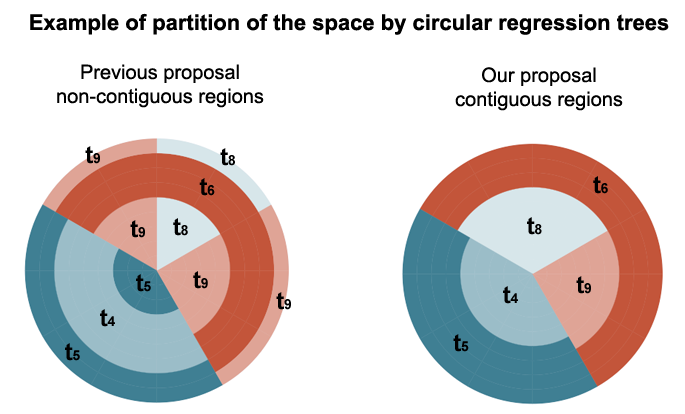
\includegraphics[width=.4\textwidth]{graphical_abstract.png}

Comparison of splits generated by two different versions of circular regression trees.

%}\\
\end{tabular}
}

\end{table*}

\clearpage
\thispagestyle{empty}

\ifpreprint
  \vspace*{-1pc}
\else
%  \vspace*{-6pc}
\fi

\begin{table*}[!t]
\ifpreprint\else\vspace*{-15pc}\fi

\section*{Research Highlights (Required)}

To create your highlights, please type the highlights against each
\verb+\item+ command. 

\vskip1pc

\fboxsep=6pt
\fbox{
\begin{minipage}{.95\textwidth}
It should be short collection of bullet points that convey the core
findings of the article. It should  include 3 to 5 bullet points
(maximum 85 characters, including spaces, per bullet point.)  
\vskip1pc
\begin{itemize}

 \item A new methodology is presented to introduce circular variables in regression trees.
 
 \item The proposed algorithm can combine linear and circular variables in the same tree.

 \item The proposed methodology reduces the computational cost of the algorithm from $\mathcal{O}(n^2)$ to $\mathcal{O}(n)$.
 
  \item Splits in this tree generate only contiguous regions, which results in simpler trees and more accurate results.

 \item Experimental tests show encouraging improvements in the accuracy of the results and computational cost.
 

\end{itemize}
\vskip1pc
\end{minipage}
}

\end{table*}

\clearpage


\ifpreprint
  \setcounter{page}{1}
\else
  \setcounter{page}{1}
\fi

\begin{frontmatter}

\title{Circular regression trees revisited}

\author[1]{Pablo \snm{Rozas Larraondo}\corref{cor1}}
\cortext[cor1]{Corresponding author:
  Tel.: +61-0414090095;}
\ead{pablo.larraondo@anu.edu.au}
\author[2]{I\~naki \snm{Inza}}
\author[2,3]{Jose A. \snm{Lozano}}

\address[1]{National Computational Infrastructure, Building 143, Australian National University, Ward Road, ACT, 2601, Australia}
\address[2]{Intelligent Systems Group, Computer Science Faculty, University of the Basque Country, Paseo de Manuel Lardizabal, Donostia, 20018, Spain}
\address[3]{Basque Center for Applied Mathematics (BCAM), Mazarredo 14, Bilbao, 48009, Spain}



\received{1 May 2013}
\finalform{10 May 2013}
\accepted{13 May 2013}
\availableonline{15 May 2013}
\communicated{S. Sarkar}


\begin{abstract}
Regression trees are a popular machine-learning method for making predictions of continuous variables. Circular variables have been traditionally used in regression trees by considering them as linear variables. A methodology to generate regression trees that understands circular variables was introduced by Lund in 2006. Lund's method recursively splits a circular space generating non-contiguous regions, requiring a $\mathcal{O}(n^2)$ computational cost. In this paper, we introduce a new methodology for incorporating circular variables into regression trees where the computational cost is reduced to $\mathcal{O}(n)$. We propose a new methodology for producing contiguous splits in circular regression trees, inspired in the way linear regression trees operate. A series of experiments demonstrates this gain in computational efficiency and accuracy when compared to both linear and previous proposals of circular regression trees. This methodology is especially suitable for training trees or ensembles of trees using large data sets that include circular variables.
\end{abstract}

\begin{keyword}
\MSC 41A05\sep 41A10\sep 65D05\sep 65D17
\KWD circular statistics\sep regression trees\sep time series\sep machine learning

%% MSC codes here, in the form: \MSC code \sep code
%% or \MSC[2008] code \sep code (2000 is the default)
\end{keyword}

\end{frontmatter}

%%\linenumbers

%% main text
\section{Introduction}
\label{intro}
Circular data are prevalent in many scientific domains, such as earth sciences, ecology or medicine. Circular data are present in any directional measurement or variable with an inherent periodicity. Wind direction, angles in molecules or time stamped data are examples of circular data.

Most of the current regression machine learning algorithms are focused on modelling the relationships between linear variables. Circular variables have a different nature to linear variables, so traditional methodologies cannot be applied or lead to wrong results in most of the cases.

A decision tree is a predictive model in which a data set is recursively partitioned based on values of the input variables, leading to smaller partitions used to estimate the target variable. A binary tree is a tree data structure in which each node has either two children or none. Classification and Regression Trees (CART) \citep{Breimanetal1984} is one of the most popular versions of binary decision trees to perform regressions. \citep{Lund2002}, introduces a methodology that demonstrates how circular variables can be incorporated into regression trees. The concept of circular regression trees substantially differs from the CART model, introducing a higher complexity and computational cost in the learning phase. 

Regression trees have been a popular and effective technique in forecasting linear variables, because of their simplicity and fast training characteristics. As the size of scientific data sets rapidly grows, there is an urgent need to come up with efficient algorithms that are able to cope with this growth. This paper proposes a different methodology to incorporate circular variables into regression trees, reducing the computational cost of Lund's proposal from $\mathcal{O}(n^2)$ to $\mathcal{O}(n)$. This methodology equates the treatment of circular variables to that of linear variables in the CART model. This results in a simpler algorithm and more accurate results.

This paper is structured as follows: Section 2 contains a detailed description of different ways of generating regression trees for linear and circular variables. The section ends with a comparison between the original and proposed methodology for building circular regression trees. Section 3 contains a series of experiments that compare efficiency and accuracy figures for classic linear regression trees and both versions of circular regression trees. Section 4 contains the conclusions and proposes further lines of investigation.


\section{Circular regression trees}

A circular variable is a numerical variable whose values are constrained into a cyclical space, for example, a variable measuring angles in radians, spans between 0 and 2$ \pi $, where both values represent the same point in space. 

Circular statistics is the field of statistics that studies circular variables. Due to the different nature of circular variables, basic statistics, such as the mean or standard deviation, require different methods than those used for linear variables. For example, if the arithmetic mean formula is used to estimate the mean of the arc degrees with values 1 and 359, the result is (1 + 359)/2 = 180, which is different to the expected 0 or 360. \citep{Fisher1992} presents in his work the statistical methodologies for circular variables.

A circular variable defines a circular space. A circular space is cyclic in the sense that it is not bounded; even the notion of a minimum and maximum values does not apply. The distance between two values in the space becomes an ambiguous concept, as it can be measured in clockwise and anticlockwise directions yielding different results. For these reasons, the '$<$' and '$>$' operators are ill defined in circular spaces.

Circular Regression Trees is a concept proposed by Lund \citep{Lund2002} to introduce circular covariates in regression trees. Lund, in his paper, builds upon Breiman's earlier work on Classification and Regression Trees (CART) \citep{Breimanetal1984}. Lund discusses the particularities of circular variables and designs a methodology to create regression trees that can combine categorical, linear and circular variables.

Lund bases his argument on the lack of meaning that '$<$' and '$>$' operators have, when applied to a circular space. These operators, used on a circular variable, only define a sense of traversing a cyclic space. The definition of a single value $\alpha$ inside a circular space does not delimit two separate regions. The variable $x$ in $(x < \alpha)$ and $(x > \alpha)$ refers to the same region, the full circle, traversed in different sense. Lund proposes instead to define regions using the '$\in$' and '$\notin$' operators, to create a recursive partitioning of a circular space. 

This approach succeeds in incorporating circular variables to regression trees, but requires a higher computational cost to generate the tree and also poses some challenges in the way it creates variable splits. In the following sections, circular regression trees will be discussed and a new way of building regression trees combining linear and circular variables will be proposed. The next subsection explores the differences and effects that the use of these two sets of operators have on classic linear regression trees. Later, the concept of circular regression tree will be introduced. Lund's proposal will be compared with the proposed new methodology to build circular regression trees. The third and last subsection discusses the differences between Lund's and our methodology, comparing their efficiency and the accuracy of the results.

\subsection{Building linear regression trees}

Regression trees, as presented by \citep{Breimanetal1984}, are built from a learning sample of observations. Let us consider a sample of observations $\mathcal{L}$ of linear variables $ X_1, X_2, \dots, X_n $ as a set of vectors $\bf{x} $ $= (x_1, x_2, \dots, x_n)$. In regression, a case consists of data $(\bf{x},$ $y)$ where $\bf{x}$ denotes measurement vectors, and $ y $ refers to the response or dependent variable. The measurement space $\mathcal{X}$ contains all possible measurement vectors. Each measurement vector in the observations sample can be represented as a point in the defined measurement space of dimension $n$. Different methods of regression analysis provide different functions $d(\bf{x})$, to estimate a value of the response variable $y$.

CART defines a way of selecting the best binary split at each non-terminal node, as well as a $d(\bf{x})$ function that provides the output at terminal nodes of a tree. These splits recursively divide the measurement space $\mathcal{X}$ in two parts. Using the '$<$' and '$>$' operators, $\mathcal{X}$ is divided along the axis of one of the covariates $X_i$ each time.

Figure \ref{f1} contains a reproduction of the example used by Breiman to represent the partition of the measurement space $\mathcal{X}$ performed by a regression tree.

% For two-column wide figures use
\begin{figure}
% Use the relevant command to insert your figure file.
% For example, with the graphicx package use
  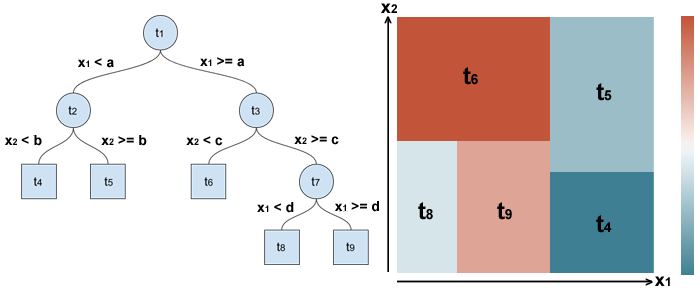
\includegraphics[width=9cm]{fig1_master.png}
% figure caption is below the figure
\caption{Example of a classic linear regression tree and a representation of how the space is divided. }
\label{f1}       % Give a unique label
\end{figure}
%
 
As can be seen in Figure \ref{f1}, nodes $t1$ and $t7$ of the sample tree select $x_1$ axis values, to split the space in two halves. Similarly, $t2$ and $t3$ select $x_2$ axis values to divide the space.

Linear regression trees recursively partition the space, finding the best split at each non-terminal node, by selecting a value which divides the space above and below. The measurement space $\mathcal{X}$ is divided in two halves by that value, along the axis of the selected covariate. To determine the best split at a node, CART only needs to identify one value for one of the covariates.

Although CART provides a methodology to easily divide the measurement space at the nodes of a tree, this is not the only way of doing it. The use of different operators, such as those proposed by Lund ('$\in$' and '$\notin$'), will result in a different partition of the space. The $in$ '$\in$' and $not in$ '$\notin$' notation comes from the set theory. It can also be used to denote whether a value belongs to a determined range within a linear space. Using a similar sample of observations to the previous example, Figure \ref{f2} shows an example of how the measurement space is divided using the new operators.

%
% For two-column wide figures use
\begin{figure}
% Use the relevant command to insert your figure file.
% For example, with the graphicx package use
  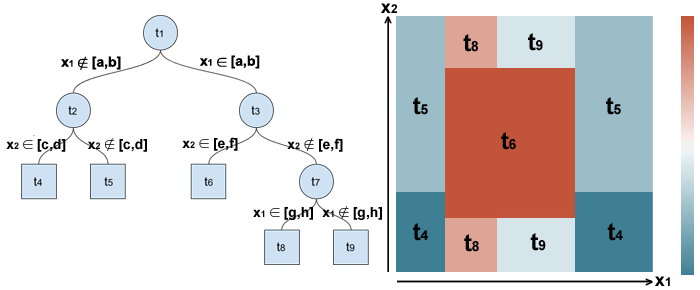
\includegraphics[width=9cm]{fig2_master.png}
% figure caption is below the figure
\caption{Example of a linear regression tree that uses the '$\in$' and '$\notin$' operators and a representation of how the space is divided.}
\label{f2}       % Give a unique label
\end{figure}
%

The most noticeable difference between the last two figures is that the resulting regions defined by the tree are spatially contiguous in Figure 1 whereas some of the equivalent regions appear as non-contiguous in Figure \ref{f2}. This new way of dividing the space requires finding a range of values within the variable’s space. The split is determined by whether values belong to that range. Finding a range instead of a value is also a perfectly valid proposal, but has computational implications, which will be discussed in Section 3.3, and depending on the data set, it can also have a negative impact on the accuracy of the resulting tree.

\subsection{Building circular regression trees}

This section considers how circular variables can be assimilated by regression trees. Lund's proposition to introduce ranges, solves the problem of univocally defining a region within a circular space. If $\alpha$ is a circular variable defined in $[0, 2\pi]$, a range within that variable can be determined by $arc(\alpha_1, \alpha_2)$. The '$\in$' and '$\notin$' operators are used to designate two regions of the circular space that belong and do not belong to that range, respectively. These two regions represent two complementary and non-overlapping regions in the circular space.

To illustrate how a circular tree partitions the space, a similar example to the one shown in the previous subsection is used. In this case, the tree contains one linear variable $x$ and one circular variable $\alpha$. Instead of using a Cartesian reference system to represent the partitions, a polar coordinate system is used to represent the circular nature of $\alpha$. Similarly to how splits for linear trees were presented, Figure \ref{f3} depicts the partitions performed by a sample circular tree.

%
% For two-column wide figures use
\begin{figure}
% Use the relevant command to insert your figure file.
% For example, with the graphicx package use
  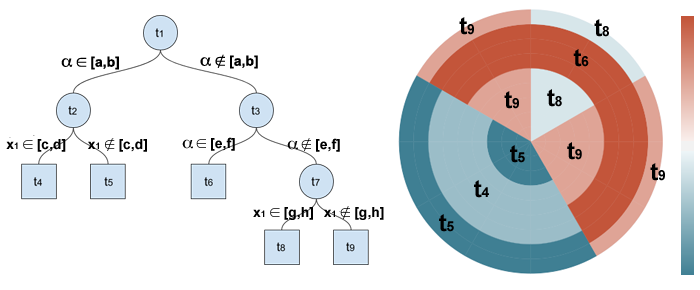
\includegraphics[width=9cm]{fig3_master.png}
% figure caption is below the figure
\caption{Example of a circular regression tree as formulated by Lund and a representation of how the space is divided.}
\label{f3}       % Give a unique label
\end{figure}
%


Figure \ref{f3} shows an example of how a circular tree partitions the space defined by one linear and one circular variables. As in Figure \ref{f2}, the space is divided in non-contiguous regions along both its axes. In this example, node $t_9$ contains data corresponding to four different regions of the space, which might limit the possibilities of finding subsequent good splits, as the correlation between these regions might not be as high as the one found in a contiguous region for other variables. 

Non-contiguous splits generate partitions in which distant parts of a data set are aggregated into the same node. For example, Figure \ref{f3} displays data corresponding to node $t_5$ split at both ends of axis $x_1$. Intuitively, data inside these two separated regions might not be as well correlated as the data delimited by a single contiguous region. As a consequence, nodes containing non-contiguous splits might degenerate in accuracy for successive partitions, when compared to contiguous splits. For the same figure, data belonging to node $t_9$ is partitioned in four different regions. Therefore, the deeper a node is in a tree, the more non-contiguous regions it produces.

The split on space performed by the '$>$' and '$<$' operators in classic linear regression trees can be seen as a particular case of the more general range selection performed by the '$\in$' and '$\notin$' operators in circular trees. The former assumes the bounds of the space to remain constant and finds a value within its range to split it in two contiguous regions. The latter finds an inner sub-region contained in a space, by identifying two delimiter values. These two values also define an outer sub-region, one at each side of the inner one, which is therefore non-contiguous.

The process described in Section 3.1, based on the '$>$' and '$<$' operators, can be seen as a particular case of the more general search in the space performed by the '$\in$' and '$\notin$' operators. Any contiguous split can be seen as a subset in which one of its bounds is shared with the original space. Partitioning the space by using the '$\in$' and '$\notin$' operators generates all the contiguous and non contiguous splits. By considering more options, it has better chances of finding a good partition, at the expense of more computations. The next subsection provides a quantitative comparison between the computational cost of building trees using contiguous and non-contiguous splits.

For any circular variable, two values are required to define two separate regions. Its first split divides the circular space in two complementary arcs. Once these limits have been defined, values within an arc can be sorted by defining one direction (clockwise or counterclockwise) of traversing the space. Having a sortable space means that the '$>$' and '$<$' operators acquire meaning, and splits can be generated by selecting just one value within an arc.

Non-contiguous spaces appear in circular trees as a consequence of using the same '$\in$' and '$\notin$' operators for subsequent splits of a circular variable. After the first split of a circular variable, once regions have been defined, the splitting method used by classic regression trees can be used to generate contiguous partitioned spaces. This is the essential difference between our proposal and Lund's version of circular regression trees and is the main contribution of this work.

Figure \ref{f4} is a graphical representation of our proposed methodology that generates contiguous circular trees applied to the same example data set. The benefits of generating contiguous splits in regression trees are discussed in the next section, considering differences in computation efficiency and accuracy.

%
% For two-column wide figures use
\begin{figure}
% Use the relevant command to insert your figure file.
% For example, with the graphicx package use
  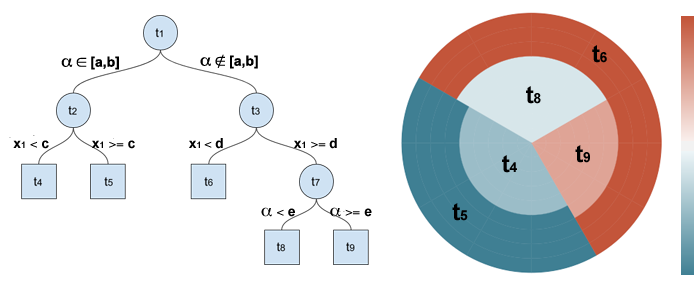
\includegraphics[width=9cm]{fig4_master.png}
% figure caption is below the figure
\caption{Example of the proposed circular regression tree and a representation of how the space is divided.}
\label{f4}       % Give a unique label
\end{figure}
%


\subsection{Comparison between contiguous and non-contiguous splits: efficiency and accuracy.} 

Optimising resources when analysing big data sets is of high interest nowadays, in order to reduce costs and execution times. There are several approaches for training trees using data sets that do not fit in the system memory \citep{Rokach2016}, such as SPRINT \citep{Shareretal1996}, SLIQ \citep{Mehtaetal1996} or FastC4.5 \citep{Heetal2007}. Most of the current efficient tree implementations are built upon the principles presented by these algorithms.

The building process of a regression tree can be separated into two phases: growth and prune. In the growth phase, the space is recursively partitioned, defining nodes until the stop criterium is satisfied. The cost of evaluating splits in linear regression trees is dominated by the computational cost of sorting values \citep{Shareretal1996}. All possible splits are considered and evaluated, using a cost function to identify the best split. This operation has a computational cost of $\mathcal{O}(n)$.

Classic linear regression trees use a methodology which divides the space in two halves each time, by selecting one value within the range of its variables. Dividing the space into two halves by selecting one value is different to having to find a subset contained anywhere within the range. This requires traversing the space considering all the possible combinations of the start and end bounds for the subset. This operation is much more expensive and has a quadratic complexity $\mathcal{O}(n^2)$.

Just the difference in the computational cost of these two splitting methods justifies the approach followed by linear regression trees when efficiency matters. In the next section, some experiments are carried out to compare the accuracy of both methodologies.

As demonstrated in the previous subsection, finding inner regions by defining both values for its boundaries, leads the tree to recursively fragment the space in non-contiguous regions. Figure 5 shows an example where the space defined by a variable is recursively split, in a tree generating non-contiguous regions.

%
% For two-column wide figures use
% \begin{figure*}
% Use the relevant command to insert your figure file.
% For example, with the graphicx package use
%  \includegraphics[width=1.0\textwidth]{image002.png}
% figure caption is below the figure
% \caption{Example of recursive space fragmentation as a result of the use of non-contiguous splits.}
% \label{fig:5}       % Give a unique label
% \end{figure*}
%

Characterising the number of non-contiguous regions at each node is not an intuitive task. It depends on the number of nodes inherited from its parent node and on how the new split is made. This number is bounded by 1 and $l$, where $l$ represents the depth level of the node in the tree, starting at its root.

A consequence of this is that for deep trees, (with a large number of levels), the fragmentation level at some nodes is substantial. This contrasts with the case of linear regression trees, where each node contains just one contiguous region of the original data set at any level. Fragmentation of the space contained by nodes comes at the price of increasing the computational cost, memory consumption and complexity of the algorithm that generates the tree.

Efficient implementations of classic linear regression trees optimise memory consumption by storing references to regions of the original data set at each node. This model has the benefit that only one copy of the data set is stored in memory. If the data set is stored in the form of pre-sorted columns, each node only has to keep two references: the minimum and maximum values of the variable, as in SPRINT \citep{Shareretal1996}.

Fragmentation of the space forces the tree structure to keep track of the boundaries for each region. This increases the complexity of nodes and raises memory use proportionally to the number of fragments in the node. Many research efforts have been made in the field of disjoint set unions, and there are many strategies than can help to structure and optimise its computational efficiency \citep{Galil1991}. Nonetheless, working with contiguous regions makes unnecessary any optimisation of the algorithms and provides a simpler solution. Table \ref{t1} compares the number of non-contiguous regions stored by a particular node for different levels of a tree, considering contiguous and non-contiguous regions.

% For tables use
\begin{table}[t]
\caption{Comparison of the growing complexity of tree nodes.}\label{t1}
\begin{center}
\begin{tabular}{rrrr}
\hline\hline
$Tree\ Level$ & $Max\ Contig$ & $Max\ Non-Contig$\\
\hline
$1$ & $0$ & $0$\\
$2$ & $2$ & $4$\\
$3$ & $2$ & $6$\\
$4$ & $2$ & $8$\\
... & ... & ...\\
$n$ & $2$ & $2n$\\

\hline
\end{tabular}
\end{center}
\end{table}

Our proposed methodology for building circular trees generates only contiguous regions with their splits. This is also a characteristic of how classic linear regression trees partition the space. It is therefore oriented to achieve maximum efficiency and can scale up for use in ensemble algorithms. Its main benefit is that the computationally expensive operation of finding the optimal subset for a circular variable, $\mathcal{O}(n^2)$, is only performed once (the first time the variable is used). All subsequent splits for that variable will be computed with $\mathcal{O}(n)$ cost. Producing contiguous regions in the splits means that the complexity of the nodes is constant, and concepts and implementations designed for linear regression trees can be easily applied.

The accuracy of a tree's results depends on how well the partitioned space represents the correlations between its variables. As was pointed out in the previous section, non-contiguous splits provide more options to partition the space, improving the chances of finding a better partition. Regression trees use a greedy algorithm in which each node selects the best split individually, without considering how the split generalises for subsequent splits. A tree selects a non-contiguous split at one of its nodes because the correlation between the values of the considered variable is higher than any of the contiguous splits. How non-contiguous splits can generalise along a tree highly depends on the data set and the relationships between its variables.


\section{Experimental evaluation}

\subsection{Data sets}

To compare the differences in accuracy between the previously discussed methods, we perform a series of experiments based on two data sets which contain circular variables. The first data set, comes from the Orbital Variations and Insolation Database \citep{Berger1991}. It contains data on changes in the earth's orbital parameters, and the resulting variations in insolation. The movements described by these parameters are commonly known as the Milankovitch cycles \citep{Hays1976}. The second data set contains meteorological data for several airports in Europe. This data set has been assembled combining numerical simulated data from the Global Forecast System model (GFS) \citep{CampanaCaplan2005} and observational data from Meteorological Aerodrome Reports (METAR) \citep{WMO1995}.

These two data sets are used to compare the differences in accuracy and and computational efficiency for the three regression methodologies discussed in this manuscript: linear, circular contiguous and circular non-contiguous trees. Each of these methodologies is used to partition each data set when predicting one of its variables. The errors and the compute times of the different trees are measured at different depths tree to compare their accuracy and computational efficiency.

\subsection{Experiment description}

The hypothesis of this study is that our proposed methodology for generating circular regression trees provides better accuracy at any depth level than both the classic linear regression tree and the previous proposal of circular regression trees. Further, since our methodology splits circular variables into contiguous regions, the search space is substantially reduced and the compute times are reduced significantly than Lund's proposal of circular tree.

In order to prove the previous statement, a general version of regression tree is implemented where each of the input variables can be tagged as \{"linear", "circular"\} and \{"contiguous", "non-contiguous"\}. These two tags indicate the kind of data and split methodology to be applied when computing the tree respectively. Classic regression trees are characterised by the pair of tags ["linear", "contiguous"], Lund's methodology by ["circular", "non-contiguous"] and our proposed methodology by ["circular", "contiguous"].

The stop criterium for all trees is based on the number of elements in a node. Splits are performed recursively until the number of data entries in a node falls below a certain value. Then, the splitting process is stopped and the node is denoted as leaf. This parameter receives the name of ”maximum leaf size”. Large values of ”maximum leaf size” generate shallow trees, whereas small values will generate deep trees with a large number of partitions. The tree implementation used to perform these experiments offers 'maximum leaf size' as one of its input parameters.

To evaluate the differences in accuracy between each of these tree methodologies, a 5-fold cross validation procedure is used. The accuracy of each tree is measured by computing the root mean squared error (RMSE) of the class variable in each row compared to the mean of the members contained in the corresponding child node of the tree. To avoid differences in the results caused by considering different partitions during the validation process, the same partition is used to test all three methodologies.

Fully grown trees may lose some generalisation capabilities, which is also known as overfitting. \citep{Kotsiantis2013} Comparing the RMSE accuracy levels at different depths provides insight on the quality of the partitions and allows detecting when accuracy starts degrading. It is considered a good characteristic of trees to produce good partitions at any level. Regression trees are a versatile algorithm which can be applied to many different problems and data sets, therefore they should provide the best possible accuracy at any depth level.

Using the data sets described above, we measure RMSE and CPU time to grow a tree, for the different versions and for a range of "maximum leaf size" values.

\subsection{Orbital variations data set}
The Orbital Variations and Insolation Database contains the values of the eccentricity, obliquity and orbital precession of the earth for the last 5 million years. Each of these parameters completes a cycle with a fixed period and the position of the earth at any particular moment is determined by the combination of all three. The earth takes around 41.000 years to complete an obliquity cycle and 26.000 year to complete a precession one. Extracting the angle phases of these two parameters and considering them as circular variables, we try to predict the values of solar radiance at 65 degrees north of latitude in July, parameter also contained in the data set.

Precession and obliquity phases are used as input variables. Each tree generates splits on the dataset based on these two variables to predict solar radiation values. The whole data set contains around 3300 roes and the "maximum leaf size" values used to generate the different versions of each tree are: 2500, 1250, 500 and 250.

\begin{table*}[t]
\caption{RMSE in predicting Radiation Levels at 65°N and CPU time to complete for the different 'max leaf size' values and versions of regression trees.}\label{t4}
\begin{center}
\begin{tabular}{crrrrrrrr}
\hline\hline
$Tree\ Version$ & \multicolumn{8}{|c|}{Max Leaf Size}\\
$$ & \multicolumn{2}{|c|}{2500} & \multicolumn{2}{|c|}{1250} & \multicolumn{2}{|c|}{500} & \multicolumn{2}{|c|}{250}\\
$$ & $RMSE$ & $T$ & $RMSE$ & $T$ & $RMSE$ & $T$ & $RMSE$ & $T $\\
\hline
Linear & 0.913 & 1 & 0.833 & 2 & 0.357 & 2 & 0.230 & 3\\
Proposed & 0.620 & 3 & 0.372 & 5 & 0.233 & 5 & 0.206 & 6\\
Lund's & 0.620 & 3 & 0.389 & 7 & 0.357 & 9 & 0.340 & 14\\
\hline
\end{tabular}
\end{center}
\end{table*}

\begin{figure}
  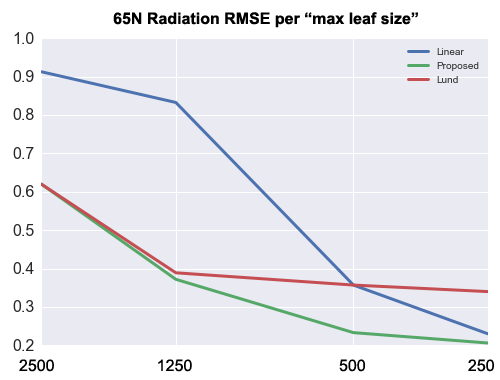
\includegraphics[width=8cm]{milankovitch_fig.png}
  \caption{RMSE values in predicting solar radiation as a function of precession and obliquity phases and "maximum leaf size".}
\label{f_tbn}
\end{figure}

Table \ref{t4} contains the resulting RMSE values and CPU times for each tree and Figure \ref{f_tbn} represents the evolution of the RMSE value as the size of the maximum leaf parameter is decreased.

\subsection{Airports meteorology data set}

The weather provides an excellent source of data for testing different machine learning algorithms. Weather data sets usually contain several variables which can be characterised as circular, such as wind direction or time and date. Using statistical methods to improve numerical weather models accuracy based on observational data is a common practice and represents an active area of research \citep{Larraondoetal2014, Salamehetal2009}.

To compare the differences between the previously discussed methods, we use meteorological data sets corresponding to seven different airports. Combining the data from GFS and METARs, four data sets are produced, containing different forecasted and observed weather variables for the airports of Barcelona (LEBL), Beijing (ZBAA), Berlin (EDDT) and Paris (LFPG). Three hourly data is collected for the years 2011, 2012 and 2013, giving approximately 8760 samples per airport. The variables contained in these data sets are: 2 metres temperature from the METAR reports and 10 metres wind speed from the GFS model. Every row in the data set has a timestamp with date and time of the values. 

Each tree generates partitions to predict observed METAR observed Temperature based on the input variables: 10 metres Wind Speed from the GFS model Date and Time. 
The input variables Date and Time are transformed into their angular numerical values so that they can be used as circular variables. The following values of "maximum leaf size" are used as inputs to the tree generation process: 2500, 1000, 500, 250, 100, 50.

\begin{table*}[t]
\caption{RMSE in predicting the observed METAR wind speed and CPU time for the different airports using the different versions of regression trees.}\label{t5}
\begin{center}
\begin{tabular}{ccrrrrrrrrrrrr}
\hline\hline
$Airport$ & $Tree\ Version$ & \multicolumn{12}{|c|}{Max Leaf Size}\\
$$ & $$ & \multicolumn{2}{|c|}{2500} & \multicolumn{2}{|c|}{1000} & \multicolumn{2}{|c|}{500} & \multicolumn{2}{|c|}{250} & \multicolumn{2}{|c|}{100} & \multicolumn{2}{|c|}{50}\\
$$ & $$ & $RMSE$ & $T$ & $RMSE$ & $T$ & $RMSE$ & $T$ & $RMSE$ & $T$ & $RMSE$ & $T$ & $RMSE$ & $T$\\
\hline
LEBL & Linear  & 3.505 & 2 & 2.884 & 3 & 2.543 & 4 & 2.402 & 4 & 2.368 & 5 & 2.361 & 6\\
LEBL & Proprosed  & 3.370 & 4 & 2.639 & 6 & 2.500 & 7 & 2.386 & 8 & 2.343 & 10 & 2.348 & 11\\
LEBL & Lund's & 3.141 & 5 & 2.597 & 7 & 2.600 & 14 & 2.573 & 14 & 2.553 & 14 & 2.555 & 14\\
\hline
ZBAA & Linear  & 5.963 & 2 & 4.772 & 3 & 4.203 & 3 & 3.911 & 5 & 3.689 & 6 & 3.679 & 8\\
ZBAA & Proposed  & 5.563 & 4 & 4.399 & 5 & 3.880 & 7 & 3.635 & 8 & 3.549 & 11 & 3.551 & 14\\
ZBAA & Lund's & 5.163 & 5 & 4.181 & 7 & 3.927 & 9 & 3.921 & 12 & 3.923 & 16 & 3.922 & 19\\
\hline
LFPG & Linear  & 4.708 & 2 & 4.073 & 3 & 3.898 & 4 & 3.797 & 5 & 3.764 & 6 & 3.767 & 8\\
LFPG & Proposed  & 4.615 & 4 & 4.078 & 6 & 3.897 & 6 & 3.765 & 9 & 3.730 & 11 & 3.737 & 13\\
LFPG & Lund's & 4.513 & 5 & 4.070 & 8 & 3.916 & 11 & 3.885 & 14 & 3.880 & 18 & 3.889 & 19\\
\hline
EDDT & Linear  & 5.166 & 2 & 4.452 & 3 & 4.275 & 4 & 4.147 & 5 & 4.119 & 7 & 4.120 & 8\\
EDDT & Proposed & 4.973 & 4 & 4.362 & 5 & 4.232 & 6 & 4.094 & 9 & 4.074 & 12 & 4.076 & 14\\
EDDT & Lund's & 4.854 & 5 & 4.374 & 7 & 4.266 & 10 & 4.157 & 15 & 4.137 & 18 & 4.138 & 22\\
\hline
\end{tabular}
\end{center}
\end{table*}

\begin{figure}
  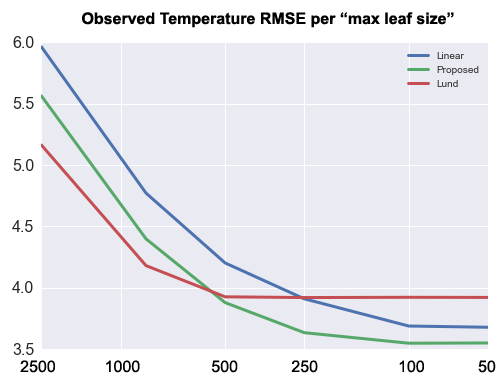
\includegraphics[width=8cm]{airports_fig.png}
\caption{RMSE values for the airport of Beijing comparing the accuracy of the output for different maximum leaf sizes.}
\label{f_tbn2}
\end{figure}

Table \ref{t5} contains the resulting RMSE values and CPU times for each tree and Figure \ref{f_tbn2} represents the evolution of the RMSE value as the size of the maximum leaf parameter is decreased.

\subsection{Analysis of experimental results}

Tables \ref{t4} and \ref{t5} contain the RMSE values and CPU times for the experiments performed on the orbital and meteorological data sets previously discussed.

Looking at the RMSE values first, it can be noted that for large values of "maximum leaf size" both circular methodologies outperform the classical linear one. When progressing into deeper levels of the tree, all three methodologies show a gain in accuracy but at different paces. Lund's method shows the best accuracy results for the first splits. However, the rate at which accuracy improves gets flat at mid depths, resulting in poorer results for the deeper trees when compared to the other two methodologies. 

This difference in the behaviour of Lund's methodology comes from its non-continuous splits generation. As previously discussed non-contiguous splits broaden the search space of the tree but come with the problem of the poor generalisation of the fragmented partitions in further splits. Figure \ref{f3} contains a graphical representation of this fact, in which some nodes contain data spread between different regions. Partitioned data are usually less correlated than contiguous and provides a worse generalisation of the containing subset. 

A non-parametric Friedman test is used to control the variability between methodologies. The RMSE results from both data sets are grouped into two categories: shallow and deep trees. The shallow group contains "max leaf size" values of [2500, 1250] for the Radiation data set and [2500, 1000] for the airport meteorology one. The deep category is formed by sizes [500, 250] of the first data set together with [500, 250, 100, 50] from the second.

For each category, the methodology proposed by \citep{Demsar2006} is used to assess the statistical significance of the differences between algorithms. For each category, the methodology proposed by \citep{Demsar2006} is used to assess the statistical significance of the differences between algorithms. The null hypothesis of similarity is rejected for each leaf size; this justifies the use of post-hoc bivariate tests (Nemenyi test, in our case), which assess the statistical difference between pairs of algorithms. The results of this test can be graphically expressed using Critical Difference (CD) diagrams.

The Nemenyi test pairwise compares every methodology. The accuracy of two methodologies is significantly different if the corresponding average rank differs by at least the critical difference. Figure \ref{f7} contains a representation of the results of the Nemenyi test comparing RMSE results for the three methodologies, one test for the case of shallow trees and another one for deep trees. These tests have been performed using the \textit{scmamp} R package publicly available at the Comprehensive R Archive Network (CRAN) \citep{Calvo2015}. Figure \ref{f7} represents the results of this test for a significance level $ p < 0.05 $ making use of CD diagrams.  These diagrams connect the groups of algorithms that are not significantly different, or in other words, whose distance is less than the critical difference, shown above the graph. As can be seen in the diagrams shown in Figure \ref{f7}, the proposed methodology outperforms the other two. Note that higher ranked algorithms in CD diagrams imply lower RMSE values.

Tables \ref{t4} and \ref{t5} also contain the CPU times to train the different versions of trees. The linear method shows the best computational efficiency results. The search space for this method is smaller than the one considered by the circular methods. The proposed methodology has the overhead of considering a bigger search space of $\mathcal{O}(n^2)$ the first time it splits a circular variable. This overhead can be assumed as a constant once all input circular variables have been split and further splits are performed in comparable times $\mathcal{O}(n)$ to the linear version. Lund's methodology, on the other hand considers the extended space for circular variables each time. This implies extra computational times of $\mathcal{O}(n^2)$ at any depth of the tree, so the differences in computational time with the linear and proposed methods will grow as deeper trees are considered.

It is worth mentioning that execution times are highly dependent on the architecture of the computer executing the code. The CPU times represented in Table \ref{t4} correspond to a desktop with a 3.2 GHz Intel Core i3 processor. The ratios between CPU times for the different experiments should be in the same order, regardless of the execution environment.

The main improvement in our methodology over the previous circular trees is that once a circular variable has been selected to create a split in a node, all subsequent splits traverse that variable in linear time instead of quadratic. The sooner circular variables are used to generate splits in a tree, the more efficient it will be. Data sets containing circular variables which are poorly correlated to the target variable require long computations, as they will not be used to create splits at any node of the tree.


\begin{figure}
\centering
\parbox{5cm}{
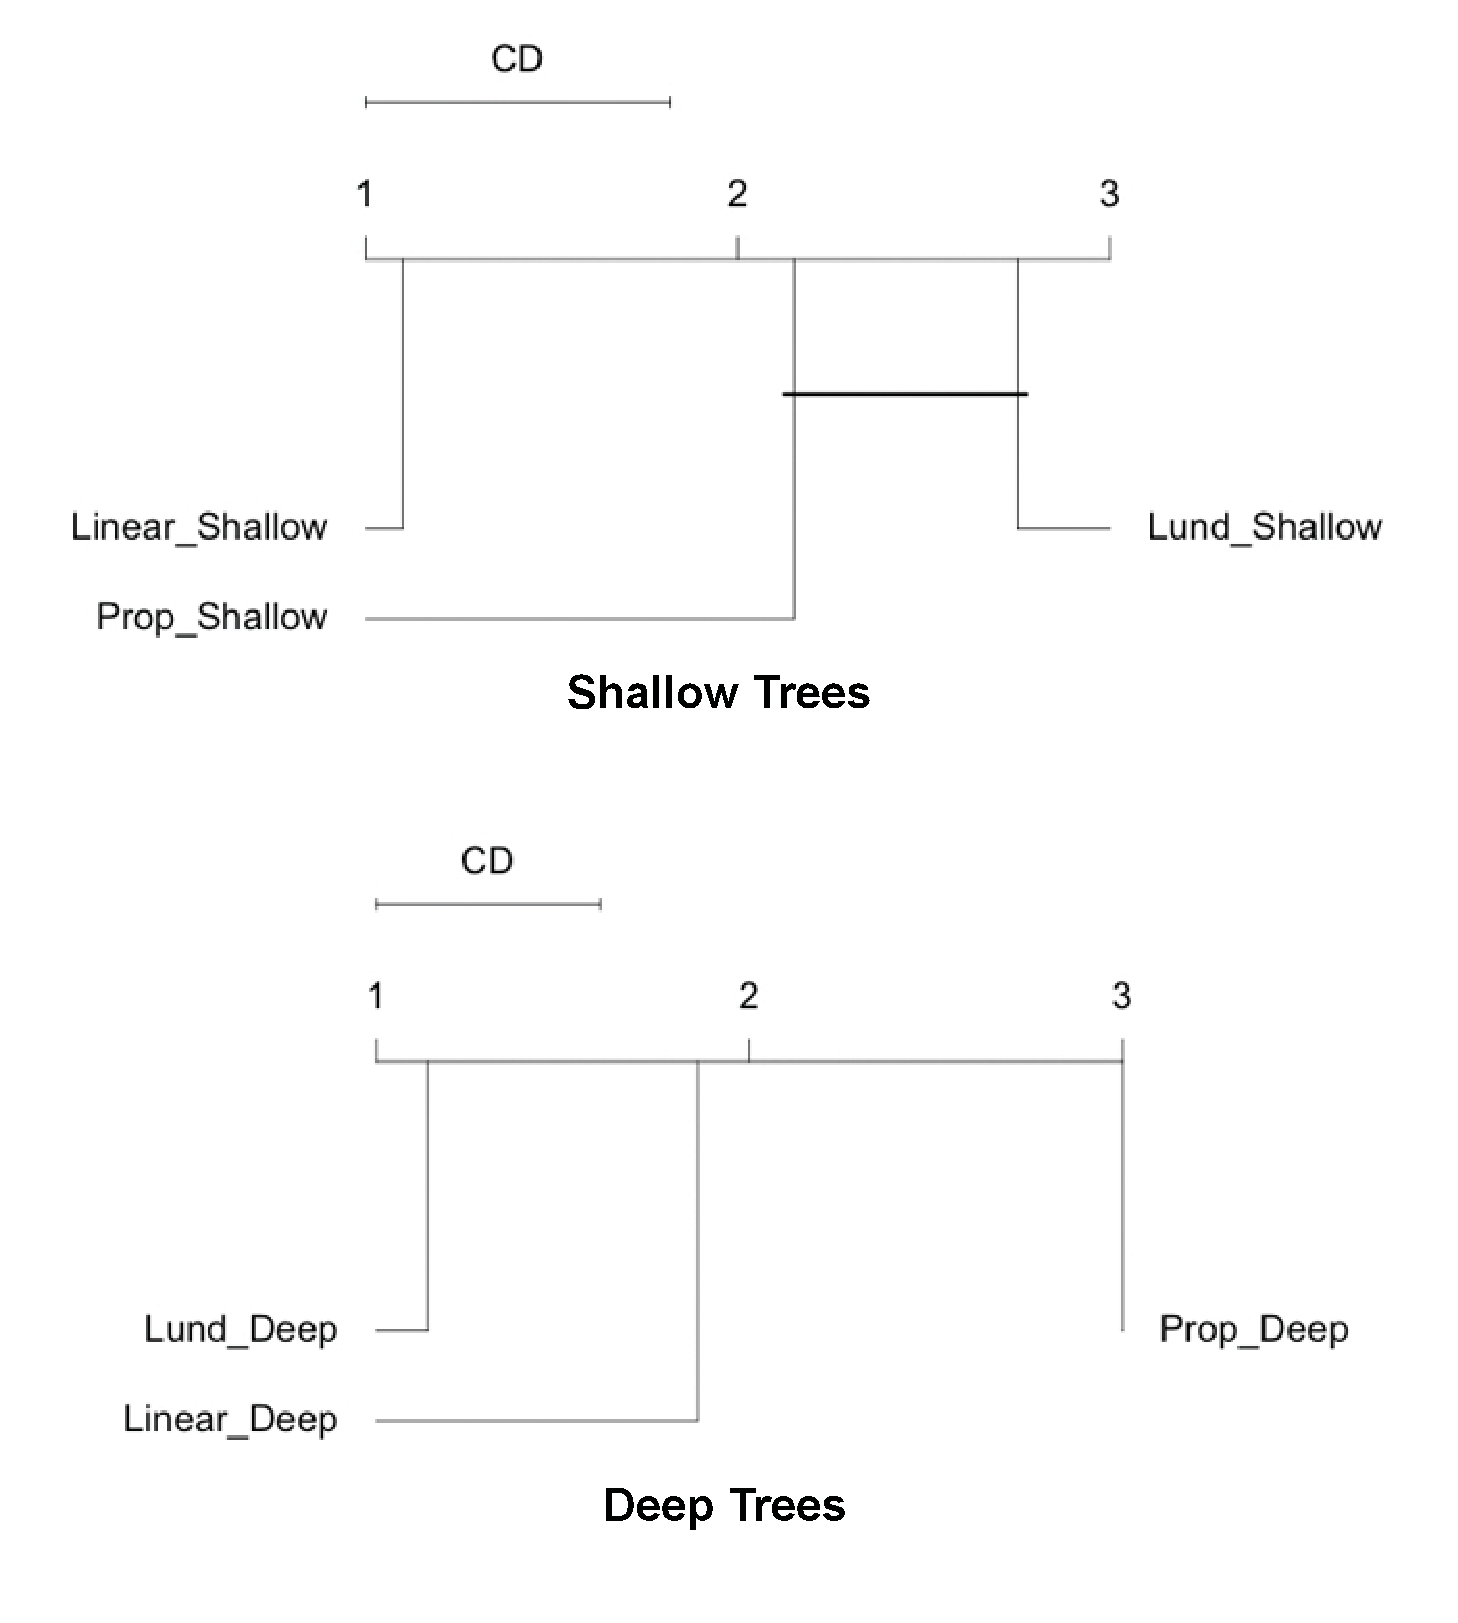
\includegraphics[width=6cm]{CD.pdf}}
\qquad
\caption{Critical Difference figures comparing the three methodologies for the case of shallow and deep trees.}
\label{f7}
\end{figure}

\section{Conclusion and Future Work}
\label{sec:5}
This work revisits the idea of circular regression trees, presenting a new methodology that improves accuracy and computational efficiency. Our proposal introduces the novelty of creating contiguous splits for the circular variables in a regression tree. The concept of the splits generating contiguous regions is inspired by how classical regression tree fragment the space. Despite non contiguous splits being a more expressive way of partitioning a data set, they can suffer from poor generalisation. Contiguous splits also benefit from improved computational efficiencies.

This paper explores the fundamental differences in partitioning the space used by regression trees. Regression trees have evolved with the introduction of many different techniques to improve efficiency. Well known techniques such as pruning, balancing, smoothing \citep{Breimanetal1984, Quinlan1993} or ensembles \citep{Buhlmann2012} can remarkably improve the accuracy of results when compared to basic regression trees.

Future work could introduce the ideas presented in this paper into more advanced implementations of regression trees. Creating contiguous splits in circular variables is an analogous process to that followed with linear variables. Existing implementations of regression trees could be adapted to compute circular trees by introducing the mechanism of tagging circular variables and computing the first split by dividing the circular space into two bounded regions. Subsequent splits can be performed using traditional methodology.

Each data set is different and normally it is a challenge to identify a methodology that performs well in every possible case. Non-contiguous splits can still be a good option and can better capture the relationships between different variables in some cases. This applies not only to circular variables but also to linear ones. An interesting line of research could be to identify scenarios where non-contiguous splits have a benefit over contiguous ones.


\section*{Acknowledgements}

We thank the Australian National Computational Infrastructure and the University of the Basque Country for their support and advice in carrying out this research work.

We are grateful for the support of the Basque Government (IT609-13, ElkartekBID3A), the Spanish Ministry of Economy and Competitiveness (TIN2013-41272-P) and a University-Society Project (15/19 – Basque Government and UPV/EHU). 

Jose A. Lozano is also supported by BERC program 2014-2017 (Basque Gov.) and Severo Ochoa Program SEV-2013-0323 (Spanish Ministry of Economy and Competitiveness).


\bibliographystyle{model2-names}
\bibliography{refs}


\section*{Supplementary Material}

The code used to run the experiments is available at:

\begin{verbatim}
 http://github.com/monkeybutter/circular_tree/
\end{verbatim}


\end{document}

%%
